\documentclass[a4paper,twoside]{article}

\usepackage{epsfig}
\usepackage{subfigure}
\usepackage{calc}
\usepackage{amssymb}
\usepackage{amstext}
\usepackage{amsmath}
\usepackage{amsthm}
\usepackage{multicol}
\usepackage{pslatex}
\usepackage{apalike}
\usepackage{SCITEPRESS}     % Please add other packages that you may need BEFORE the SCITEPRESS.sty package.
\usepackage{url}

\subfigtopskip=0pt
\subfigcapskip=0pt
\subfigbottomskip=0pt

\begin{document}

\title{YouPower --  A Social App for User Engagement in Power Grids
%\subtitle{Preparation of Camera-Ready Contributions to SCITEPRESS Proceedings} 
}

\author{\authorname{First Author Name\sup{1}, Second Author Name\sup{1} and Third Author Name\sup{2}}
\affiliation{\sup{1}Institute of Problem Solving, XYZ University, My Street, MyTown, MyCountry}
\affiliation{\sup{2}Department of Computing, Main University, MySecondTown, MyCountry}
\email{\{f\_author, s\_author\}@ips.xyz.edu, t\_author@dc.mu.edu}
}

\keywords{Power Grid, Energy Community, Social Participation, Social App, YouPower}

\abstract{The abstract should summarize the contents of the paper and should contain at least 70 and at most 200 words. The text must be set to 9-point font size. \vspace*{2cm}}

\onecolumn \maketitle \normalsize \vfill

\section{\uppercase{Introduction}}
\label{sec:introduction}

\noindent 
This paper presents the design of YouPower, a social smart grid platform that is designed as a means to explore the potential and challenges of supporting social participation, awareness and engagement of power gird users (\url{https://app.civisproject.eu}). The goal of developing such a system is to make energy visible, to inform users' energy know-how, to promote
pro-environmental social norms, and to facilitate users in their day-to-day life to take energy-friendly actions together with online communities. 

X The idea of linking smart grids with (online) \textit{Social Network}s (SNs) as a joint R\&D topic has recently caught
much attention in media
\cite{Boslet2010,Chima2011,Erickson2012,Fang2013}. There are many
research efforts on either topics, but research on combining SNs with
smart grids has just started. A number of recent works propose frameworks or
approaches that interconnect smart meters (or smart homes) as SNs for
energy management and sharing \cite{Ciuciu2012,Steinheimer2012}. In
addition, Silva et. al.~\cite{Silva2012} conducted surveys to
understand user needs for energy services including SN
services. Several frameworks or simulation models for demand side
management and value-added web services with SN aspects have been
developed~\cite{Chatzidimitriou2013,De-Haan2011,Lei2012}. Others have
used simulation models to demonstrate the feasibility of social
coordination in supply and demand \cite{Skopik2014,Worm2013}.
% 
Our research interest expands on the related work in that it focuses
on smart grid user communities. The research is performed within the
framework of the EU FP7 CIVIS
project (\url{www.civisproject.eu}).

Project Context 


\begin{figure*}[t!]
\begin{center}\footnotesize
	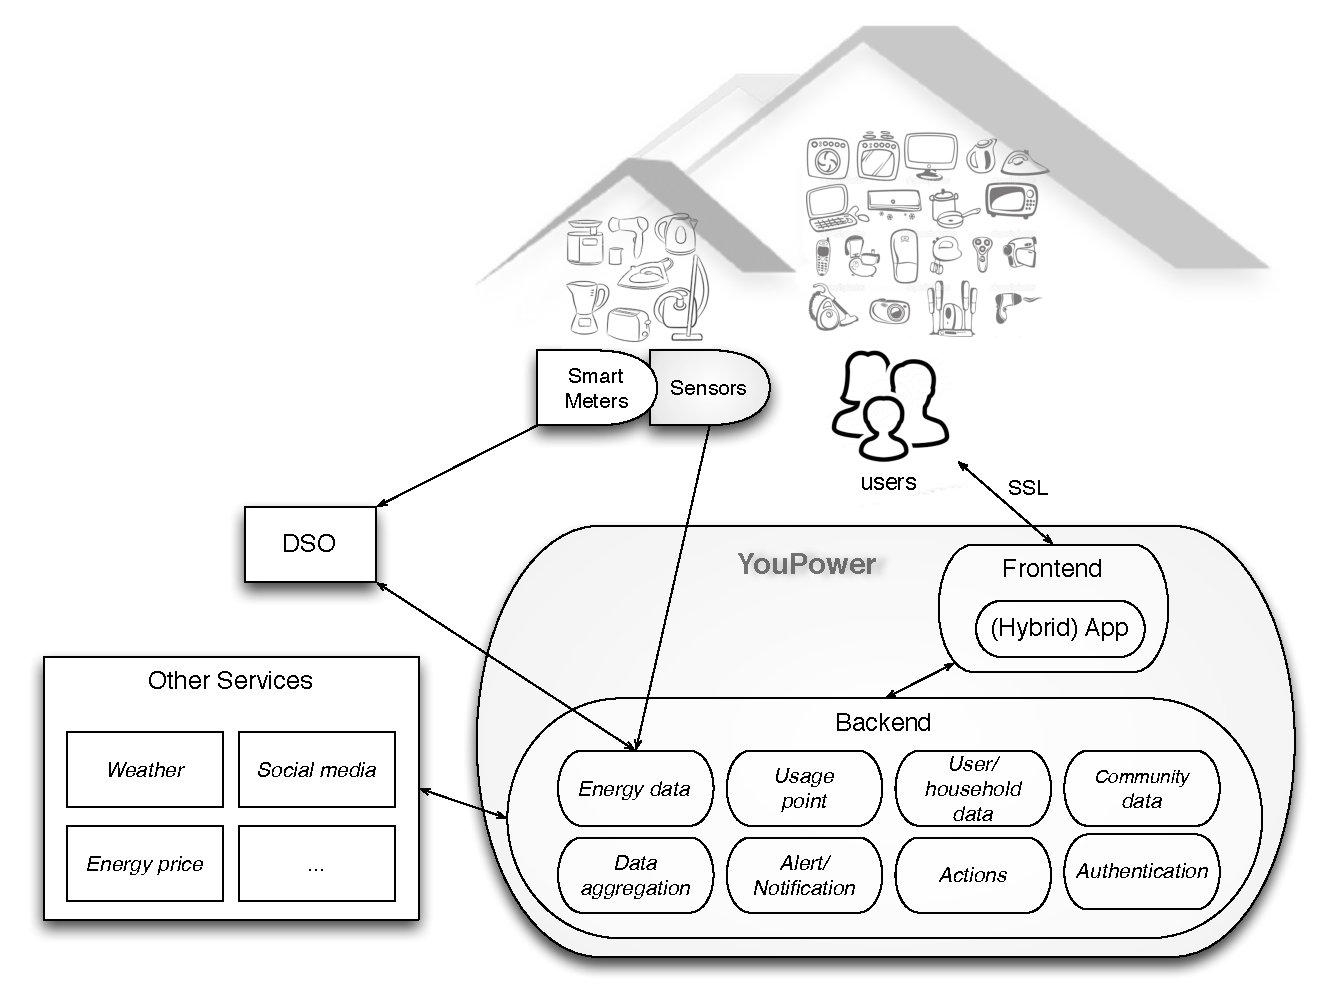
\includegraphics[width=.7\textwidth]{img/civis_platform_overview.pdf}\\
	DSO (Distribution System Operators),  SSL (Secure Sockets Layer)
	\caption{YouPower system overview}\label{fig:platform}
\end{center}
\end{figure*}

\section{\uppercase{State of the Art}}



\noindent X Considering the analytical frames and the CIVIS use cases, we chose a set of platform features and translated those into three self-contained and composable parts to be included in the CIVIS (front-end) application (hereinafter abbreviated as CIVIS app)\footnote{A shortened list of YouPower app mock-ups can be found at \url{http://civis.tbm.tudelft.nl/mockups/}.}: 
%\begin{enumerate}
%\item \nameref{sect:tips}
%\item \nameref{sect:brf}
%\item \nameref{sect:load_shifting}
%\end{enumerate}



With peer review results and users' feedback on the design, adaptations and changes are made to suit user needs and to achieve the CIVIS research goal. 
In general, the application aims to enhance users' energy know-how through action suggestions that are implementable in everyday life, engage users in energy communities with understandable and actionable information and feedback, and facilitate community interaction and self-teaching by means of group discussions.
%

Given the time and resource constraints, the app can not be developed all-in-one cross-platform (for phones, tablets and computers). We chose to design the front-end as a mobile app. This means that the app design has layouts and user interactions that suit (small) phone screens. %The consideration is multi-fold. 
Western Europe has a large mobile phone internet user base\footnote{
Between 2013 and 2017, the penetration rate of mobile phone internet users among mobile phone users will rise from 49.0\% to 77.8\%. See more at:\url{ http://www.emarketer.com/Article/Nearly-Half-of-Western-Europeans-Will-Use-Mobile-Web-This-Year/1010510\#sthash.AaVfsqIU.dpuf}}. Many surveys show that mobile apps have advantages such as creating deeper user engagement, easy sharing, among others\footnote{\url{https://infomedia.com/blog/the-advantages-of-mobile-apps/}, \url{https://econsultancy.com/blog/62326-85-of-consumers-favour-apps-over-mobile-websites/}}. This makes mobile app a good choice given the goal of the CIVIS platform. Once developed, mobile apps can also be more easily transformed to web browser versions, while the reverse is more difficult. The back-end of the CIVIS platform will remain mostly the same independent of the front-end alternatives. 


\section{\uppercase{Design Concept}}
\label{sect:design_concept}

\subsection{Action Suggestions}
\label{sect:tips}

This part of YouPower aims to provide users easy access to practical and inexpensive suggestions (or tips) to (1) increase energy awareness, (2) inform energy know-how, and to (3) shape their long-term behaviors related to household energy consumption.
% 
We collected about 50 suggestions (\url{https://goo.gl/R11QdZ}) from credible sources such as national and international energy agencies and associations. There are routine actions such as ``don't keep hot water flowing when you wash your dishes by hand'', regular actions such as ``defrost your fridge in $x$ days'', and one time actions such as ``install a programmable thermostat''.  
Each action is accompanied with a short explanation that mainly focuses on intrinsic values to target long-term sustainable behaviors, the estimated impact and entailed effort (on a scale of 1 to 5), and the information about how many users are taking the action. 

Users can choose to take a few actions at a time and are suggested with a new action when one is completed. 
Some suggestions can be triggered by time, e.g., ``defrost your fridge in $x$ days.'' In such cases, the app reminds the users of the pending actions they are interested in. 
%A user has an ``action list'' that registers the user's actions. 
%
When an action is completed, the user is awarded with points (displayed as \textit{Leaves}) associated to the effort and impact level of that action. 
A user may also choose to abandon or reschedule an accepted action. 
Upon action completion and cancellation, a user is asked to give feedback. 
The user may ``like'' and ``share'' an action, rate the effort level of the action and give comments. 

%\begin{figure}
%\begin{center}
%	\begin{minipage}[t]{0.44\textwidth}
%	   \frame{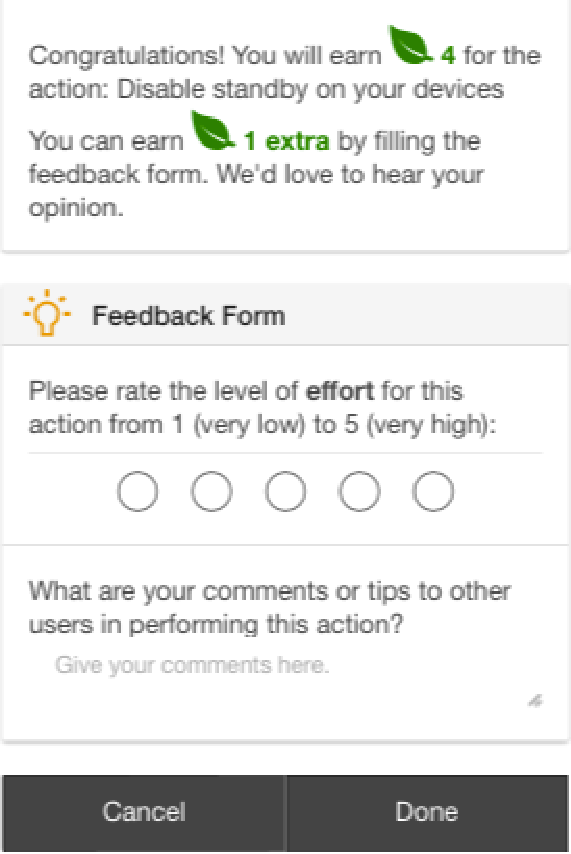
\includegraphics[width=\textwidth]{img/action_completed.pdf}}
%	    \caption{The feedback form when a user completes an action.}\label{fig:action_completed}
%	  \end{minipage}
%	  \hfill
%	\begin{minipage}[t]{0.44\textwidth}
%	   \frame{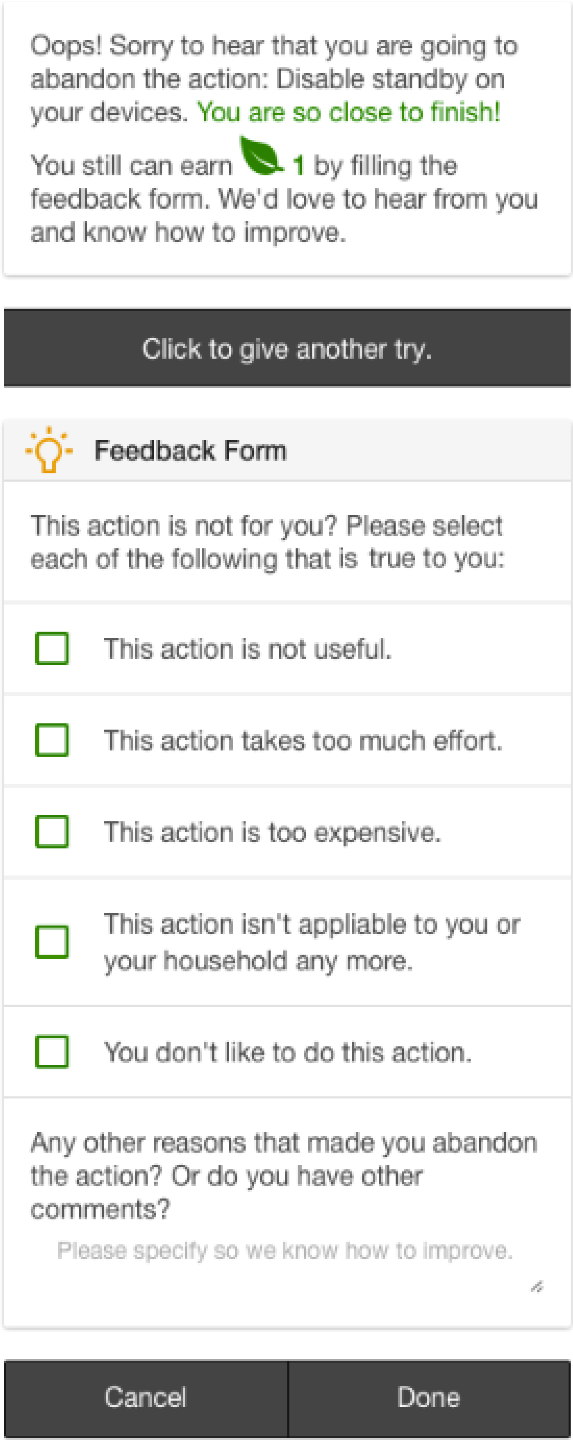
\includegraphics[width=\textwidth]{img/action_not_completed.pdf}}
%	   \caption{The feedback form when a user abandons an action.}\label{fig:action_not_completed}
%	  \end{minipage}
%\end{center}
%\end{figure} 

\paragraph{Engagement in Household and Communities} 
To engage each member in a household, the app allows a user to add members (who are also YouPower users) to his/her household. 
A user can see the actions of household members, and add their actions to his/her own action list.
% 
A user can also join communities and participate in discussions to exchange their ideas and share experiences. The top actions (the ones with most participants) in a community are displayed to members to introduce social norms. 


%This application allows users to create and participate in community and personal energy challenges. It gives participants feedback on their performance during the challenge period and provides encouragement for participation using micro-actions. Users who performed well can share their success stories with other users. The application also allows for friends and group discussion. The community challenges can be incentivised by local investments (solar panels for the building), or through funding projects in developing countries (a school in Uganda). This application tries to motivate user engagement in energy community.

%\paragraph{Feedback on Achievements}
%In order to keep users motivated, we implement a set of achievements that are unlocked over time by using the app and performing the actions. For instance, users can get an achievement notification after they have performed a certain number of actions, accumulated a certain number of leaves individually or as part of some community, or after they have been using the app regularly for a certain period of time. Whenever a user unlocks an achievement in some category, s/he gets informed what is the next achievement in this category that s/he can reach. (E.g. ``Congrats! You completed your first $3$ actions! Your next goal is $5$ actions. Keep it up!'') Such achievements are based on the goal-setting \cite{Abrahamse2007265} and individual and collective feedback \cite{Abrahamse2013} approaches to behavioral changes in energy consumption.

\paragraph{Personalization and Localization}
A user has a personal profile and a household profile. We allow a user to customize the display name, preferred language (English, Italian or Swedish), and to provide information about the household composition, home type and size, major appliances, etc. The information is useful for personalized action suggestions, the comparison of similar households and individuals, and can be used for research purposes. A user (at the test sites) can link YouPower to the household's (DSO and sensors) energy data if an data account is provided. 
% 
In such cases, the app customizes its content to a user's test site: housing cooperatives content for the Swedish site and load-shifting content for the Italian site. They are discussed in the next two subsections. 


\paragraph{Design Evaluation}
The design was evaluated by peer reviews, a study with 24 participants 
in an environmentally-oriented event in Helsinki (\url{https://oscedays.org/helsinki/}), 
and a workshop with nine participants in the Italian test site. 
% 
In general, people liked the idea of receiving action suggestions. 
They like to see the impact of their actions and asked for easy to perform actions. 
The majority was interested in collaborative community actions, e.g., to save together and to donate for a common goal. Very few had interest in competition. 
% 
% Some people mentioned that the connection (or difference) between the \textit{Suggestions} and the \textit{Challenges} is hard to understand. Challenges were designed to express personal or community energy-goals, while suggestions are the means to achieve the goals. We later changed the name of this feature from \textit{Challenges} to \textit{Achievements}. 
% 
%Some people asked for the authority of the suggestions: it isn't clear where the tips come from. To what extent can they be trusted? Are they results of applied research? This is not marginal in a community of people who are quite familiar with energy-related issues. Having an explanation of how trustworthy these tips are would be very important. 
%%
%The meaning and value of the leaves are also another aspect that was questioned the most. 
%We thus decided to have an information page so that a number of such issues can be explained to the users. 
%In addition, users can send feedback to CIVIS through the app to keep the designers updated of users' concerns, questions, or other issues. 
% 
Many expressed the opinion that monetary savings are only somewhat important to them. They were also skeptical about how much money they can actually save. They instead showed interest to learn about energy saving strategies as they are driven by more intrinsic motives.
% 
Some participants think that the others (in their neighborhood or city) do not put the same effort in energy conservation as themselves do. The YouPower approach to display other people's actions may have the potential to motivate people seeing the others' efforts.
%
Some suggested that for those who do not have or are not comfortable with smart-phones, the app should be made available through a browser. 


\subsection{Housing Cooperatives}
\label{sect:brf}

This part of YouPower is considered for households in the Stockholm test site. In Sweden, each apartment or house owner is a member of a housing cooperative that owns the property and annually elects a board that is in charge of the finances and maintenance of the property including making energy related decisions. 
Such a housing ownership concept exists in a number of EU and non-EU countries.
% 
Three main categories of features are designed for this part of YouPower: energy information about a user's own housing cooperative, energy information about other housing cooperatives, and support for communication between energy managers.
Primary users are energy managers and board members of housing cooperatives. Secondary users are ordinary cooperative members. 

Housing cooperative energy information includes comparative energy performance %(kWh /m$^{2}$)\footnote{We chose to use kWh in this case since cooperative managers have fairly good knowledge of energy units and the visualization is comparative.} 
and the cooperative's monthly and yearly energy use, divided into heating (including hot water) and facilities electricity. Energy actions that have been taken are listed in relation with energy consumptions. 
A user can see when different actions, such as energy information, optimisation or investments, were previously taken and see more details about the actions. By comparing the energy use with previous periods, the user can also see the impact of the actions.
% 
In the same way that the users can view information about their own cooperatives, they can also see the energy performance and energy actions taken by other cooperatives. This allows energy managers and others who are interested to e.g. explore the effect of a neighbouring cooperative's actions on their energy use and read about how they carried out an investment and which contractor was used. 
% 
To further support collaboration and knowledge exchange between housing cooperatives, there is a discussion group dedicated for energy managers. Within the group they have the possibility of creating discussion topics of their interests. In this way, the discussion of the occasional meetings with the local energy network can be extended to continue online.

\begin{figure}
\centering
\includegraphics[width=0.9\linewidth]{"img/housing cooperatives 1"}
\includegraphics[width=0.9\linewidth]{"img/housing cooperatives 2"}
\caption{Mock-up of the ``housing cooperatives'' part}
\label{fig:brf}
\end{figure}

\paragraph{Design Evaluation}

The design was evaluated with three energy managers and the feedback was incorporated in the design improvement of the application. The energy managers would primarily want to use the app to find housing cooperatives with similar challenges and see what actions they had taken. They also thought the app would be helpful for deciding which companies can be trusted based on what other housing cooperatives had done and what the effects were on the energy use. The energy managers doubted that other members in their cooperatives would be very interested in following the cooperative's energy use, but they thought the app might be useful for engaging members in specific questions. 

\subsection{Energy Data} 
\label{sect:load_shifting}

Three different levels of energy consumption data are displayed in the app: household, appliances and community. 
At the household level, the current and historical consumptions are displayed. For users with production from renewable sources, which is the case for users from the two Trentino pilot sites where many have roof-installed PV panels, the app compares production and consumption levels with the aim to raise awareness of different prosumption patterns and to maximize self-consumption. 
% 
For users with installed smart plugs, the app visualizes consumption patterns at the single appliance level. This is meant to enable users to gain a deeper understanding of the relationship between their daily actions and the resulting energy consumption. 
%
At the community level, aggregated data is displayed on the energy balance of a community. In Italy test sites, community refers to a whole electric consortium, while in Sweden the housing cooperative a user belongs to. 
In particular, data on the aggregated monthly consumption and production levels is reported, together with monthly trends. The overall balance in the share of self-consumption is also reported. 
%A single household's consumption level with is compared with the community average. This is meant to represent a powerful tool in helping users make sense of the actual consumption data, driving them towards the goal of a ``fair energy use''. At the same time, this can also be seen as a social mechanism, where community-level dynamics are used as a means to achieve a given goal, in this case increased energy efficiency at the single household level.

\paragraph{Dynamic Time-of-Use Tariffing}
In the Trento pilot site, the main focus is to leverage load elasticity for maximizing self-consumption of locally-installed Renewable Energy Sources (RESs). This means that electric loads shall be shifted to the time of high production. In order to achieve this, the lever identified has been that of price, actuated by means of a dynamic time-of-usage tariffing scheme. 
A predictive engine has been designed and implemented to predict with a good accuracy the level of production from renewables in the subsequent 72 hours. The engine, which is based on a linear prediction model, uses weather forecast data (in particular: solar radiation data) from both public and private sources~\footnote{Data from Meteotrentino (\url{http://www.meteotrentino.it/}), OpenWeatherMap (\url{http://openweathermap.org/}), Fondazione Edmund Mach (\url{http://www.fmach.it/}) and US National Weather Service (\url{http://nomads.ncep.noaa.gov/}) is used in the predictor to build the feature vector.}, and historical data about the production of single renewable plants, provided by local stakeholders CEIS and CEDIS.
Estimating also consumption patterns, based on historical data (again weighted based on environmental conditions for accounting for climate factors), a matching engine has been developed which forecasts whether there will be surplus of local production. In this case a favorable price is offered to users, as an incentive for them to move flexible loads (e.g., dishwater and washing machine) to those time intervals. At the same time, higher prices will be used to discourage usage of energy-intensive appliances when local production is low compared to consumption requests. In the app this takes the form of an indication of the foreseen price for the next 72 hours, divided into time intervals of three-hours duration each. The indication of the price for each time interval is accompanied by an icon, smiling if the price is below a given threshold (computed based on the historical price of energy in the previous two years) or presenting a sad expression otherwise. As the tariff is based on the estimated energy balance for the consumption as a whole, it is not personalised but it is the same for all local users.

\paragraph{Donation (Trento Test Site)}
CIVIS users in the Trento test site can sign up for a donation programme, organized as a crowdfunding campaign. Subscription to the donation programme is optional. In case a user signs up, his/her contribution towards a better community energy balance brings about economic benefits for the electric consortia as well. In both Trento test sites, indeed, local generation from RESs exceeds, at the aggregated yearly level, consumption needs. Yet there is a timing mismatch, so that in order to serve consumption peaks the consortia have to buy (expensive) electricity on the national energy market. At the same time there are time periods during which production exceeds consumption, so that excess energy has to be sold, typically at a much lower price, on the market.

The donation mechanism co-designed with the local stakeholder foresees that such economic benefit for the consortia will be partially monetized in order to contribute to a project with a social goal. Each project has a well-defined beneficiary. For a given project the app visualizes, besides the name of the beneficiary and a short description of the project, information on the current status of the campaign, i.e., how much money has been collected with respect to the goal. Also, a plot displaying the trend of donations for that specific campaign since the beginning is plotted.

The donation mechanism, coupled with the dynamic ToU tariffing scheme, is the key 'social' aspect foreseen for the Trento pilot site. It is based on the concept that the adoption of environmentally-friendly behaviors at the individual level can generate positive impacts at the social level ("social as a goal"). In this case impacts are on two different levels. First, in terms of reduced greenhouse gas emissions, as the local generation is totally based on RESs and hence carbon-neutral. Second, by contributing to the funding of a social project users can see a concrete, tangible effect of their action, fostering their motivation. 

The visualization of the donation programme status and trends requires such data to be made available through the WP4 platform.

\paragraph{Design Evaluation}
The design of the energy data visualization and comparison part has been validated incrementally with users in the Trentino site. Two focus groups and four workshops were conducted. During the focus group events, ideas about the possible functionalities were used as probes with the participants. During the workshops, practical activities were carried out with the participants in order to develop an idea of the most desirable features and then to receive evaluation feedback.
% 
One issue that emerged was the interest in the production data and the ability to maximize self-consumption. The ideas of the dynamic ToU and the donation programme were also well received. 

\section{\uppercase{Manuscript Preparation}}


\noindent {\bf Group 2.} Additionally, you may wish to copy and edit
the following 3 example files:
\begin{verbatim}
  - example.bib
  - example.tex
  - scitepress.eps
\end{verbatim}



\subsubsection{Tables}

\begin{table}[h]
\caption{This caption has more than one line so it has to be
justified.}\label{tab:example2} \centering
\begin{tabular}{|c|c|}
  \hline
  Example column 1 & Example column 2 \\
  \hline
  Example text 1 & Example text 2 \\
  \hline
\end{tabular}
\end{table}



%\begin{figure}[!h]
%  \vspace{-0.2cm}
%  \centering
%   {
\epsfig{file = SCITEPRESS.eps, width = 5.5cm}}
%  \caption{This caption has more than one line so it has to be justified.}
%  \label{fig:example2}
%  \vspace{-0.1cm}
%\end{figure}


\subsubsection{Equations}

Equations should be placed on a separate line, numbered and
centered.\\The numbers accorded to equations should appear in
consecutive order inside each section or within the contribution,
with the number enclosed in brackets and justified to the right,
starting with the number 1.

Example:

\begin{equation}\label{eq1}
    a=b+c
\end{equation}

\subsubsection{Program Code}\label{subsubsec:program_code}

Program listing or program commands in text should be set in
typewriter form such as Courier New.

Example of a Computer Program in Pascal:

\begin{small}
\begin{verbatim}
 Begin
     Writeln('Hello World!!');
 End.
\end{verbatim}
\end{small}


\section{\uppercase{Conclusions}}
\label{sec:conclusion}


\section*{\uppercase{Acknowledgements}}

\noindent This research is funded by the EU FP7 CIVIS project.
%It is also partly funded by the NWO project RobuSmart
%(Increasing the Robustness of Smart Grids through distributed
%energy generation: a complex network approach), grant number
%647.000.001. The authors would like to thank Jukka K. Nurminen from Aalto Univ. and Jan M�uller from KIT for their
%comments.


\bibliographystyle{apalike}
{\small
\bibliography{bib}}


%\section*{\uppercase{Appendix}}
%
%\noindent If any, the appendix should appear directly after the
%references without numbering, and not on a new page. To do so please use the following command:
%\textit{$\backslash$section*\{APPENDIX\}}

\vfill
\end{document}

